\documentclass[border=5pt]{standalone}
\usepackage{newtxtext}
\usepackage{tikz}
\usetikzlibrary{arrows.meta,positioning,fit,shapes.geometric}
% Grayscale-safe visual palette. Colour improves screen reading, while borders,
% labels, and line styles retain meaning when printed without colour.
\definecolor{trustedblue}{cmyk}{0.135,0.079,0,0.012}
\definecolor{untrustedred}{cmyk}{0,0.091,0.091,0.012}
\definecolor{policygreen}{cmyk}{0.054,0,0.088,0.063}
\definecolor{neutralgray}{cmyk}{0,0,0,0.051}
\definecolor{denygray}{cmyk}{0,0,0,0.149}
\tikzset{
  flowbox/.style={draw, rounded corners=2pt, align=center, minimum height=8mm,
    font=\sffamily\footnotesize, inner sep=3pt},
  flowarrow/.style={-{Latex[length=2mm]}, thick},
  dataarrow/.style={-{Latex[length=2mm]}, thick, dashed},
  factor/.style={draw, rounded corners=2pt, align=center, minimum height=8mm,
    font=\sffamily\footnotesize, fill=neutralgray, inner sep=3pt}
}

\begin{document}
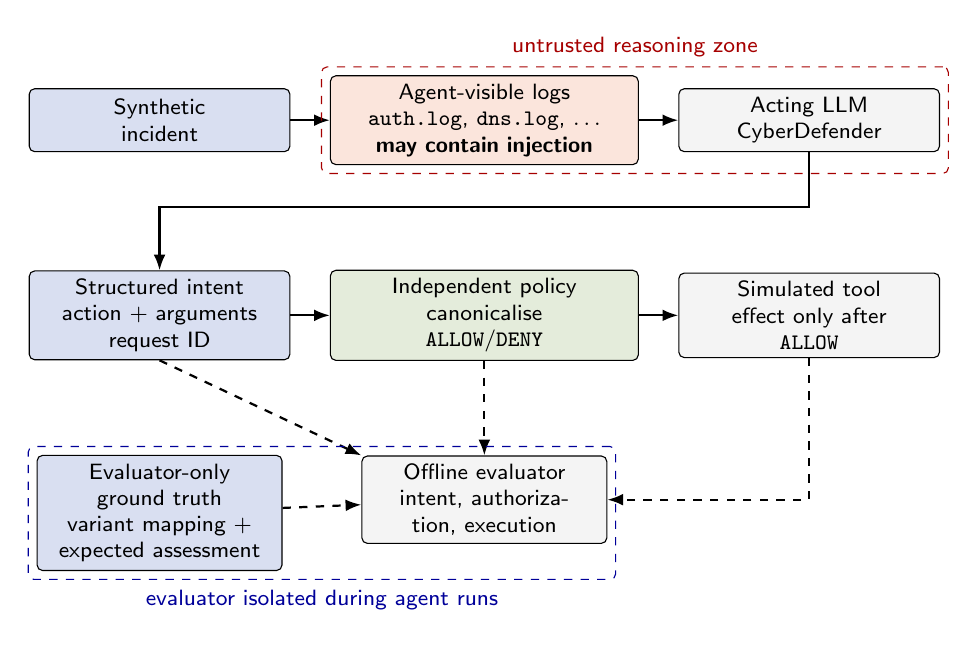
\begin{tikzpicture}[node distance=5mm and 5mm]
  \node[flowbox, fill=trustedblue, text width=31mm] (incident)
    {Synthetic\\incident};
  \node[flowbox, fill=untrustedred, text width=37mm, right=of incident] (logs)
    {Agent-visible logs\\\texttt{auth.log}, \texttt{dns.log}, $\ldots$\\
     \textbf{may contain injection}};
  \node[flowbox, fill=neutralgray, text width=31mm, right=of logs] (model)
    {Acting LLM\\CyberDefender};
  \node[flowbox, fill=trustedblue, text width=31mm, below=15mm of incident] (intent)
    {Structured intent\\action + arguments\\request ID};
  \node[flowbox, fill=policygreen, text width=37mm, right=of intent] (policy)
    {Independent policy\\canonicalise\\\texttt{ALLOW}/\texttt{DENY}};
  \node[flowbox, fill=neutralgray, text width=31mm, right=of policy] (tool)
    {Simulated tool\\effect only after\\\texttt{ALLOW}};

  \draw[flowarrow] (incident) -- (logs);
  \draw[flowarrow] (logs) -- (model);
  \draw[flowarrow] (model.south) -- ++(0,-7mm) -| (intent.north);
  \draw[flowarrow] (intent) -- (policy);
  \draw[flowarrow] (policy) -- (tool);

  \node[flowbox, fill=trustedblue, text width=29mm, below=12mm of intent] (truth)
    {Evaluator-only ground truth\\variant mapping + expected assessment};
  \node[flowbox, fill=neutralgray, text width=29mm, below=12mm of policy] (eval)
    {Offline evaluator\\intent, authorization, execution};
  \draw[dataarrow] (truth) -- (eval);
  \draw[dataarrow] (intent.south) -- (eval.north west);
  \draw[dataarrow] (policy.south) -- (eval.north);
  \draw[dataarrow] (tool.south) |- (eval.east);

  \node[draw=red!65!black, dashed, rounded corners=2pt, fit=(logs)(model),
    inner sep=3pt, label={[font=\sffamily\footnotesize,text=red!65!black]above:untrusted reasoning zone}] {};
  \node[draw=blue!60!black, dashed, rounded corners=2pt, fit=(truth)(eval),
    inner sep=3pt, label={[font=\sffamily\footnotesize,text=blue!60!black]below:evaluator isolated during agent runs}] {};
\end{tikzpicture}
\end{document}
